%\begin{comment}
\chapter{Data Validation Plots for $K_S^0$}
The full distributions of the input variables of \textit{KsFinder} are shown in the Figure A-1. The small discrepancies are observed in the distributions after applying the \textit{KsFinder} selection cut while the agreement before applying such cut is fine. The main reason is that the difference in the \textit{cosVertexMomentum} which plays the most important role in the $K_S^0$ classification. Even before the use of \textit{KsFinder}, small differences can be observed. This variable is sensitive to the $K_S^0$ vertexing quality and the VXD misalignment, which is still subject to be optimized in future. 
  
\begin{figure}[H]
\caption{The distribution of the training variables in KsFinder. The blue and purple solid lines in the top plots are the total and true $K_S^0$ distributions from generic MC, respectively. The bottom plots are the data-MC ratio before (blue) and after (red) applying \textit{KsFinder} cut.}
\begin{subfigure}{0.5\linewidth}
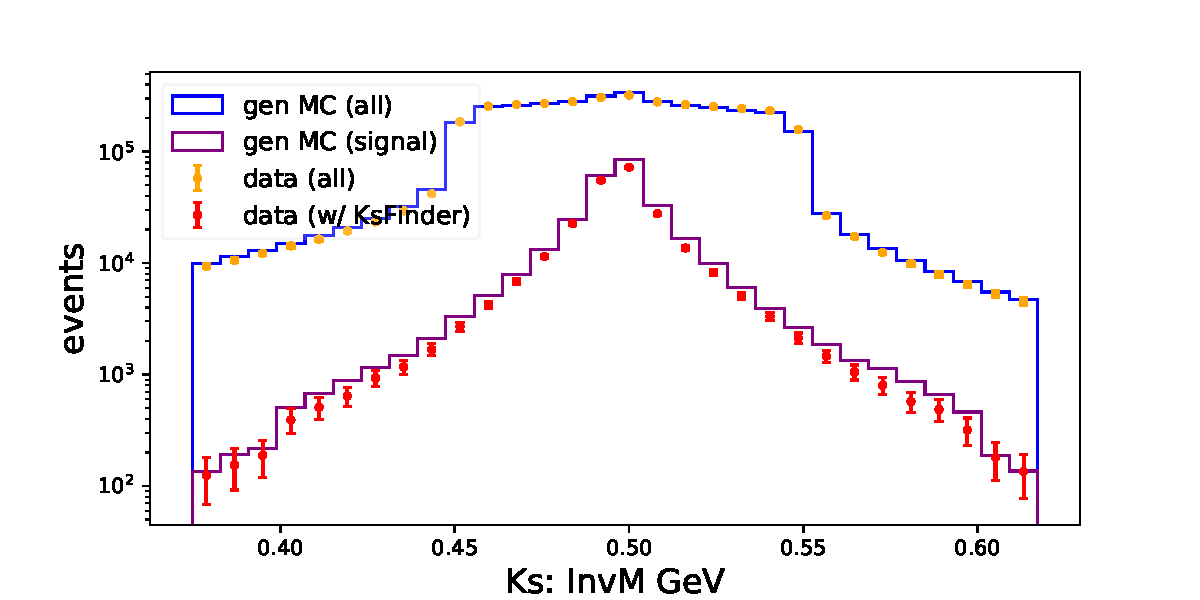
\includegraphics[page=1,width=1.1\linewidth]{dataVarsPlot_Ks.pdf}
\end{subfigure}
\begin{subfigure}{0.5\linewidth}
\includegraphics[page=2,width=1.1\linewidth]{dataVarsPlot_Ks.pdf}
\end{subfigure}
\end{figure}

%\begin{comment}
\begin{figure}[H]
\ContinuedFloat
\begin{subfigure}{0.5\linewidth}
	\includegraphics[page=3,width=1.1\linewidth]{dataVarsPlot_Ks.pdf}
\end{subfigure}
\begin{subfigure}{0.5\linewidth}
	\includegraphics[page=4,width=1.1\linewidth]{dataVarsPlot_Ks.pdf}
\end{subfigure}
\begin{subfigure}{0.5\linewidth}
	\includegraphics[page=5,width=1.1\linewidth]{dataVarsPlot_Ks.pdf}
\end{subfigure}
\begin{subfigure}{0.5\linewidth}
	\includegraphics[page=6,width=1.1\linewidth]{dataVarsPlot_Ks.pdf}
\end{subfigure}
\end{figure}

\begin{figure}[H]
\ContinuedFloat
\begin{subfigure}{0.5\linewidth}
	\includegraphics[page=7,width=1.1\linewidth]{dataVarsPlot_Ks.pdf}
\end{subfigure}
\begin{subfigure}{0.5\linewidth}
	\includegraphics[page=8,width=1.1\linewidth]{dataVarsPlot_Ks.pdf}
\end{subfigure}
\begin{subfigure}{0.5\linewidth}
	\includegraphics[page=9,width=1.1\linewidth]{dataVarsPlot_Ks.pdf}
\end{subfigure}
\begin{subfigure}{0.5\linewidth}
\includegraphics[page=10,width=1.1\linewidth]{dataVarsPlot_Ks.pdf}
\end{subfigure}
\end{figure}

\begin{figure}[H]
\ContinuedFloat
\begin{subfigure}{0.5\linewidth}
	\includegraphics[page=11,width=1.1\linewidth]{dataVarsPlot_Ks.pdf}
\end{subfigure}
\begin{subfigure}{0.5\linewidth}
	\includegraphics[page=12,width=1.1\linewidth]{dataVarsPlot_Ks.pdf}
\end{subfigure}
\begin{subfigure}{0.5\linewidth}
\includegraphics[page=13,width=1.1\linewidth]{dataVarsPlot_Ks.pdf}
\end{subfigure}
\begin{subfigure}{0.5\linewidth}
\includegraphics[page=14,width=1.1\linewidth]{dataVarsPlot_Ks.pdf}
\end{subfigure}
\end{figure}

%\begin{comment}
\begin{figure}[H]
	\ContinuedFloat
	\begin{subfigure}{0.5\linewidth}
		\includegraphics[page=15,width=1.1\linewidth]{dataVarsPlot_Ks.pdf}
	\end{subfigure}
	\begin{subfigure}{0.5\linewidth}
		\includegraphics[page=16,width=1.1\linewidth]{dataVarsPlot_Ks.pdf}
	\end{subfigure}
\begin{subfigure}{0.5\linewidth}
\includegraphics[page=17,width=1.1\linewidth]{dataVarsPlot_Ks.pdf}
\end{subfigure}
\begin{subfigure}{0.5\linewidth}
\includegraphics[page=18,width=1.1\linewidth]{dataVarsPlot_Ks.pdf}
\end{subfigure}

\end{figure}

\begin{figure}[H]
	\ContinuedFloat
\begin{subfigure}{0.5\linewidth}
	\includegraphics[page=19,width=1.1\linewidth]{dataVarsPlot_Ks.pdf}
\end{subfigure}
\begin{subfigure}{0.5\linewidth}
	\includegraphics[page=22,width=1.1\linewidth]{dataVarsPlot_Ks.pdf}
\end{subfigure}
\begin{subfigure}{0.5\linewidth}
	\includegraphics[page=23,width=1.1\linewidth]{dataVarsPlot_Ks.pdf}
\end{subfigure}
\begin{subfigure}{0.5\linewidth}
	\includegraphics[page=24,width=1.1\linewidth]{dataVarsPlot_Ks.pdf}
\end{subfigure}
\end{figure}

\begin{figure}[H]
	\ContinuedFloat
	\begin{subfigure}{0.5\linewidth}
		\includegraphics[page=25,width=1.1\linewidth]{dataVarsPlot_Ks.pdf}
	\end{subfigure}
\end{figure}
%\end{comment}

%\end{comment}

%\end{comment}
